\begin{note}
	Положим $\Omega(U) = \bigcup_{k \geq 0} \Omega^k(U)$. Тогда внешний дифференциал $d$ порождает <<послойное>> отображение $d : \Omega(U) \to \Omega(U)$. 
\end{note}

\begin{lemma}
	Для всех форм $\omega, \nu \in \Omega^k(U)$, $\tau \in \Omega^l(U)$ и $c \in \R$ выполнено:
	\begin{enumerate}[itemsep = 0pt, topsep =5pt]
		\item Линейность: $d(\omega + \nu) = d \omega + d \nu$, $d(c \omega) = c \cdot d \omega$,
		\item Правило Лейбница: $d(\omega \wedge \tau) = d \omega \wedge \tau + (-1)^k \omega \wedge d \tau$, 
		\item $d(d \omega) = 0$.
	\end{enumerate}
	Кроме того, если линейный оператор $D : \Omega(U) \to \Omega(U)$ удовлетворяет этим трем свойствам и на $f \in C^{\infty}(U)$ дает дифференциал $f$, то $D = d$.
\end{lemma}

\begin{myproof}
	Первое свойство вытекает из определения, докажем второе. 
	В силу линейности, достаточно проверить его для мономов $\omega = f dx^I$, $\tau = g dx^J$, где $I \in \mathbb{I}_k$, $J \in \mathbb{I}_l$, $f, g \in C^{\infty}(U)$. 
	По определению внешнего произведения имеем: 
	\[ d(\omega \wedge \tau) = d(fg \, dx^I \wedge dx^J) = d(fg) \wedge dx^I \wedge dx^J = (g df + f dg) \wedge dx^I \wedge dx^J. \]
	Раскроем скобки, получим слагаемые $g df \wedge dx^I \wedge dx^J = (df \wedge dx^I) \wedge (g dx^J) = d\omega \wedge \tau$ и $f dg \wedge dx^I \wedge dx^J$.
	Переставим 1-форму $dg$ и $k$-форму $dx^I$. По суперкоммутативности это дает знак $(-1)^{k}$:
	\[ f (dg \wedge dx^I) \wedge dx^J = f (-1)^k (dx^I \wedge dg) \wedge dx^J = (-1)^k (f dx^I) \wedge (dg \wedge dx^J) = (-1)^k \omega \wedge d\tau. \]
	Складывая, получаем требуемое равенство. 

	\vspace{5pt}
	Третье свойство сначала проверим для $f \in \Omega^0(U)$:
	\[ d(df) = d\left( \sum_{i=1}^m \frac{\partial f}{\partial x_i} dx_i \right) = \sum_{i=1}^m d\left( \frac{\partial f}{\partial x_i} \right) \wedge dx_i = \sum_{i, j = 1}^m \frac{\partial^2 f}{\partial x_j \partial x_i} dx_j \wedge dx_i. \]
	Эта сумма равна нулю в силу теоремы Шварца. 
	Также из определения внешнего дифференциала $\forall I \in \mathbb{I}_k : d(dx^I) = 0$, тогда для произвольного монома $f dx^I$ имеем:
	\[ d( d(f dx^I) ) = d(df \wedge dx^I) = d(df) \wedge dx^I + (-1)^1 df \wedge d(dx^I) = 0. \]
	В итоге третье свойство вытекает по линейности из доказанного. 

	\vspace{5pt}
	Пусть $D : \Omega(U) \to \Omega(U)$ удовлетворяет указанным свойствам. 
	В силу линейности достаточно установить равенство $D = d$ на мономах. 
	Так как $D$ и $d$ совпадают на гладких функциях, то $D(dx_i) = D(Dx_i) = 0$. 
	Тогда по индукции и правилу Лейбница $\forall I \in \mathbb{I}_k : D(dx^I) = 0$. 
	Следовательно, 
	\[ D(f \cdot dx^I) = D(f \wedge dx^I) = df \wedge dx^I + f \wedge D(dx^I) = df \wedge dx^I = d(f \cdot dx^I). \]
	В итоге равенство $D = d$ на $\Omega^k(U)$ вытекает по линейности из доказанного.
\end{myproof}


\begin{theorem}
	Пусть $U \subset \R^m$, $V \subset \R^n$ открыты, определена функция $f : U \to V$ класса $C^{\infty}$, тогда $\forall \omega \in \Omega^k(V) : d(f^* \omega) = f^* d \omega$. 
\end{theorem}

\begin{myproof}
	Для $g \in \Omega^0(V)$ по правилу дифференцирования композиции имеем: 
	\[ d(f^* g) = d(g \circ f) = dg \circ df = f^* dg. \]
	К тому же для каждого $I = (i_1, \dotsc, i_k) \in \mathbb{I}_k$ по правилу Лейбница и свойству $d \circ d = 0$ имеем: 
	\[ d(f^* dy^I) = d(df_{i_1} \wedge \dotsc \wedge df_{i_k}) = 0. \] 
	Следовательно, для монома $g dy^I = g \wedge dy^I$ получаем:
	\[ d (f^* (g dy^I) ) = d (f^* g \wedge f^* dy^I) = d(f^* g) \wedge (f^* dy^I) + 0 = f^* dg \wedge f^* dy^I = f^* (dg \wedge dy^I) = f^* d(g dy^I). \]
	Общий случай следует по линейности $d$ и $f^*$.
\end{myproof}


\subsection{Дифференциальные формы на многообразиях} 

Напомним, что под гладкостью понимается принадлежность классу $C^{\infty}$. 

\begin{definition}
	Пусть $M$ -- гладкое $m$-мерное многообразие в $\R^n$, $k \in \N_0$. 
	\textit{Дифференциальной $k$-формой} $\omega$ на $M$ называется функция, которая точкам $p \in M$ сопоставляет форму $\omega_p \in A_k(T_p M)$ на касательном пространстве. 
\end{definition}

\begin{definition}
	Пусть $f : M \to N$ -- гладкое отображение многообразий, $\omega$ -- $k$-форма на $N$. 
	Тогда \textit{переносом} $\omega$ называется $k$-форма $f^* \omega$ на $M$, значение которой в точках $p \in M$ определяется формулой:
	\[ \forall v_1, \dotsc, v_k \in T_p M : (f^* \omega)_p (v_1, \dotsc, v_k) = \omega_{f(p)} (df_p(v_1), \dotsc, df_p(v_k)), \]
	где $df_p : T_p M \to T_{f(p)} N$ -- дифференциал отображения $f$.
\end{definition}

\begin{note}
    Свойства линейности и уважения внешнего произведения сохраняются для многообразий.
	Также, если $g : N \to P$ -- гладкое отображение, то $(g \circ f)^* = f^* \circ g^*$.  
\end{note}

\begin{example}
	Рассмотрим вложение $i_M : M \to \R^n$, $i_M(x) = x$. 
	Если на открытом множестве $U \supset M$ в $\R^n$ задана $k$-форма $\nu$, то ее можно перенести на $M$.
	Форма $i^*_M \nu$ называется ограничением формы $\nu$ на $M$ и обозначается $\nu|_M$.
\end{example}

Определим гладкость формы в точке, сделать это можно двумя способами. 

\begin{definition}
	Форма $\omega$ называется \textit{гладкой в точке} $p \in M$, если существует такая параметризация $\phi : V \to U$ окрестности $p$ в $M$, что $\phi^* \omega \in \Omega(V)$.
\end{definition}

\begin{definition}
	Форма $\omega$ называется \textit{гладкой в точке} $p \in M$, если существует открытое в $\R^n$ множество $W \ni p$ и $\widetilde{\omega} \in \Omega(W)$, что $\omega = \widetilde{\omega}|_M$ на $W \cap M$.
\end{definition}

\begin{lemma}
	Определения гладкости формы в точке эквивалентны.
\end{lemma}

\begin{myproof}
	$(\Ra)$ Пусть выбрана параметризация $\phi : V \to U = W \cap M$, где $W$ открыто в $\R^n$, такая что $\phi^* \omega \in \Omega(V)$. 
	Уменьшая окрестности, если необходимо, можно считать, что $\phi^{-1}$ продолжимо на $W$, то есть существует гладкая функция $F : W \to V$, $F|_{W \cap M} = \phi^{-1}$. 
	Положим $\widetilde{\omega} = F^*(\phi^* \omega)$. 
	Тогда $\widetilde{\omega} \in \Omega(W)$ как перенос гладкой формы. 
	Поскольку $F \circ i_M = \phi^{-1}$ на $W \cap M$, то имеем следующую цепочку равенств на $W \cap M$:
	\[ \widetilde{\omega}|_M = i_M^* (F^* (\phi^* \omega)) = (F \circ i_M)^* (\phi^* \omega) = (\phi^{-1})^* (\phi^* \omega) = (\phi \circ \phi^{-1})^* \omega = \omega. \]

	\vspace{5pt}
	$(\La)$ Обратно, пусть $\widetilde{\omega}|_M = \omega$ на $W \cap M$. Уменьшая $W$, если необходимо, можно считать, что существует параметризация $\phi : V \to W \cap M$. 
	Тогда $i_M \circ \phi : V \to W$ и $\phi^* \omega = (i_M \circ \phi)^* \widetilde{\omega} \in \Omega(V)$, что завершает доказательство.
\end{myproof}

\begin{note}
	Из доказательства также вытекает, что в определениях кванторы существования можно заменить на кванторы всеобщности. 
\end{note}

\begin{definition}
	Форма $\omega$ называется \textit{гладкой на $M$}, если она гладкая в каждой точке $M$.
	Обозначения: $\Omega^k(M)$, $\Omega(M) = \bigcup_{k \geq 0} \Omega^k(M)$. 
\end{definition}

\begin{lemma}
	Пусть $f : M \to N$ -- гладкое отображение многообразий. Тогда перенос сохраняет гладкость, то есть $f^* : \Omega^k(N) \to \Omega^k(M)$. 
\end{lemma}

\begin{myproof}
	Пусть $\omega \in \Omega^k(N)$. 
	Для точек $p \in M$ и $q = f(p) \in N$ выберем параметризации $\phi : U_0 \to U \ni p$, $\psi : V_0 \to V \ni q$. 
	Уменьшая окрестности, если необходимо, можно считать, что $f(U) \subset V$. 
	Рассмотрим координатное представление $g : U_0 \to V_0$ по правилу $g = \psi^{-1} \circ f \circ \phi$. Тогда $\psi \circ g = f \circ \phi$. 
	Следовательно, справедливо равенство 
	$g^* (\psi^* \omega) = \phi^* (f^* \omega)$. 
	Так как $\omega$ гладкая, то $\psi^* \omega \in \Omega^k(V_0)$. Отображение $g$ гладкое как координатное представление $f$. Следовательно, по свойству переноса, форма $g^* (\psi^* \omega)$ является гладкой на $U_0$.
	Значит, $\phi^* (f^* \omega)$ тоже гладкая, что по определению означает гладкость $f^* \omega$ в точке $p$.
\end{myproof}

\vspace{5pt}
Перенесем на многообразия операцию внешнего дифференцирования.

\begin{definition}
	Пусть $\omega \in \Omega(M)$ и $\phi : V \to U$ -- параметризация окрестности $U$ в $M$. 
	Определим дифференциал $\omega$ на $U$ формулой:
	\[ d \omega : =  (\phi^{-1})^* d (\phi^* \omega). \]
\end{definition}

\begin{note}
	Покажем, что определение корректно.
	Пусть $\psi : W \to \R^n$ -- другая параметризация $M$, такая что $O = \phi(V) \cap \psi(W) \neq \emptyset$. 
	Тогда $g : \phi^{-1}(O) \to \psi^{-1}(O)$ по правилу $g = \psi^{-1} \circ \phi$ является диффеоморфизмом и $\phi = \psi \circ g$. 
	Следовательно, по теореме 7.2 на $\phi^{-1}(O)$ имеем равенства:
	\[ d(\phi^* \omega) = d(g^* \psi^* \omega) = g^* d(\psi^* \omega) = [\phi^* \circ (\psi^{-1})^*] \, d(\psi^* \omega). \] 
	Если к обеим частям применить $(\phi^{-1})^*$, то получим $(\phi^{-1})^* d (\phi^* \omega) = (\psi^{-1})^* d(\psi^* \omega)$ на $O$. 
	Следовательно, локальные определения склеиваются в глобальную форму $d \omega \in \Omega(M)$.
\end{note}

\begin{note}
	Из свойств дифференциала в $\R^n$ следует, что для $d$ на многообразии выполнены свойства 1-3 из леммы 7.4.
	Кроме того, если $f \in C^{\infty}(M)$, то $df = (\phi^{-1})^* d (f \circ \phi) = d(f \circ \phi)(d \phi^{-1})$.
	То есть определение совпадает с дифференциалом функции.
\end{note}

\begin{note}
	Возможность продолжения локального $d$ на $M$ и независимость от параметризации следуют также из единственности оператора со свойствами 1-3 из леммы 7.4.
\end{note}

\begin{theorem}
	Пусть $f : M \to N$ -- гладкое отображение многообразий, тогда для всех $\omega \in \Omega(N)$ имеем
	\[ d(f^* \omega) = f^* d \omega. \]
\end{theorem}

\begin{myproof}
	Будем пользоваться обозначениями из леммы 7.6. 
	Так как $\psi \circ g = f \circ \phi$, то по определению $d$ и свойствам переноса имеем: 
	\[ \phi^* d (f^* \omega) = d(\phi^* f^* \omega) = d((f \circ \phi)^* \omega) = d((\psi \circ g)^* \omega) = d (g^* (\psi^* \omega)) = g^* (d (\psi^* \omega)) = g^* \psi^* d \omega. \]
	Последние два равенства выполнены по теореме 7.2. Осталось заметить, что в правой части $\phi^* f^* d \omega$, откуда $d(f^* \omega) = f^* d \omega$.
\end{myproof}

\begin{corollary}
	Пусть в $\R^n$ выбрана окрестность $W \supset M$ и $\widetilde{\omega} \in \Omega^k(W)$, такая что $i^*_M \widetilde{\omega} = \omega$. 
	Тогда $d \omega = i^*_M d \widetilde{\omega}$. 
\end{corollary}





\subsection{Разбиение единицы}

 Построение начнем с функции $f : \R \to \R$, $f \in C^{\infty}(\R)$:
 \[ f(t) = \begin{cases}
  e^{-1/t}, & t > 0,  \\  
  0, & t \leq 0. 
 \end{cases} \]
 Ее свойства доказывались при изучении рядов. 
 Рассмотрим функцию $h(t) = \frac{f(R^2 - t)}{f(R^2 - t) + f(t - r^2)}$, $0 < r < R$. 
 Она тоже лежит в классе $C^{\infty}(\R)$. 
 Тогда функция $\beta : \R^n \to \R$ по правилу $\beta(x) = h(|x - x_0|^2) \in C^{\infty}(\R^n)$ для некоторой $x_0 \in \R^n$ называется функцией \textit{<<шапочка>>}.

\begin{figure}[h!]
\centering
\begin{framed}
		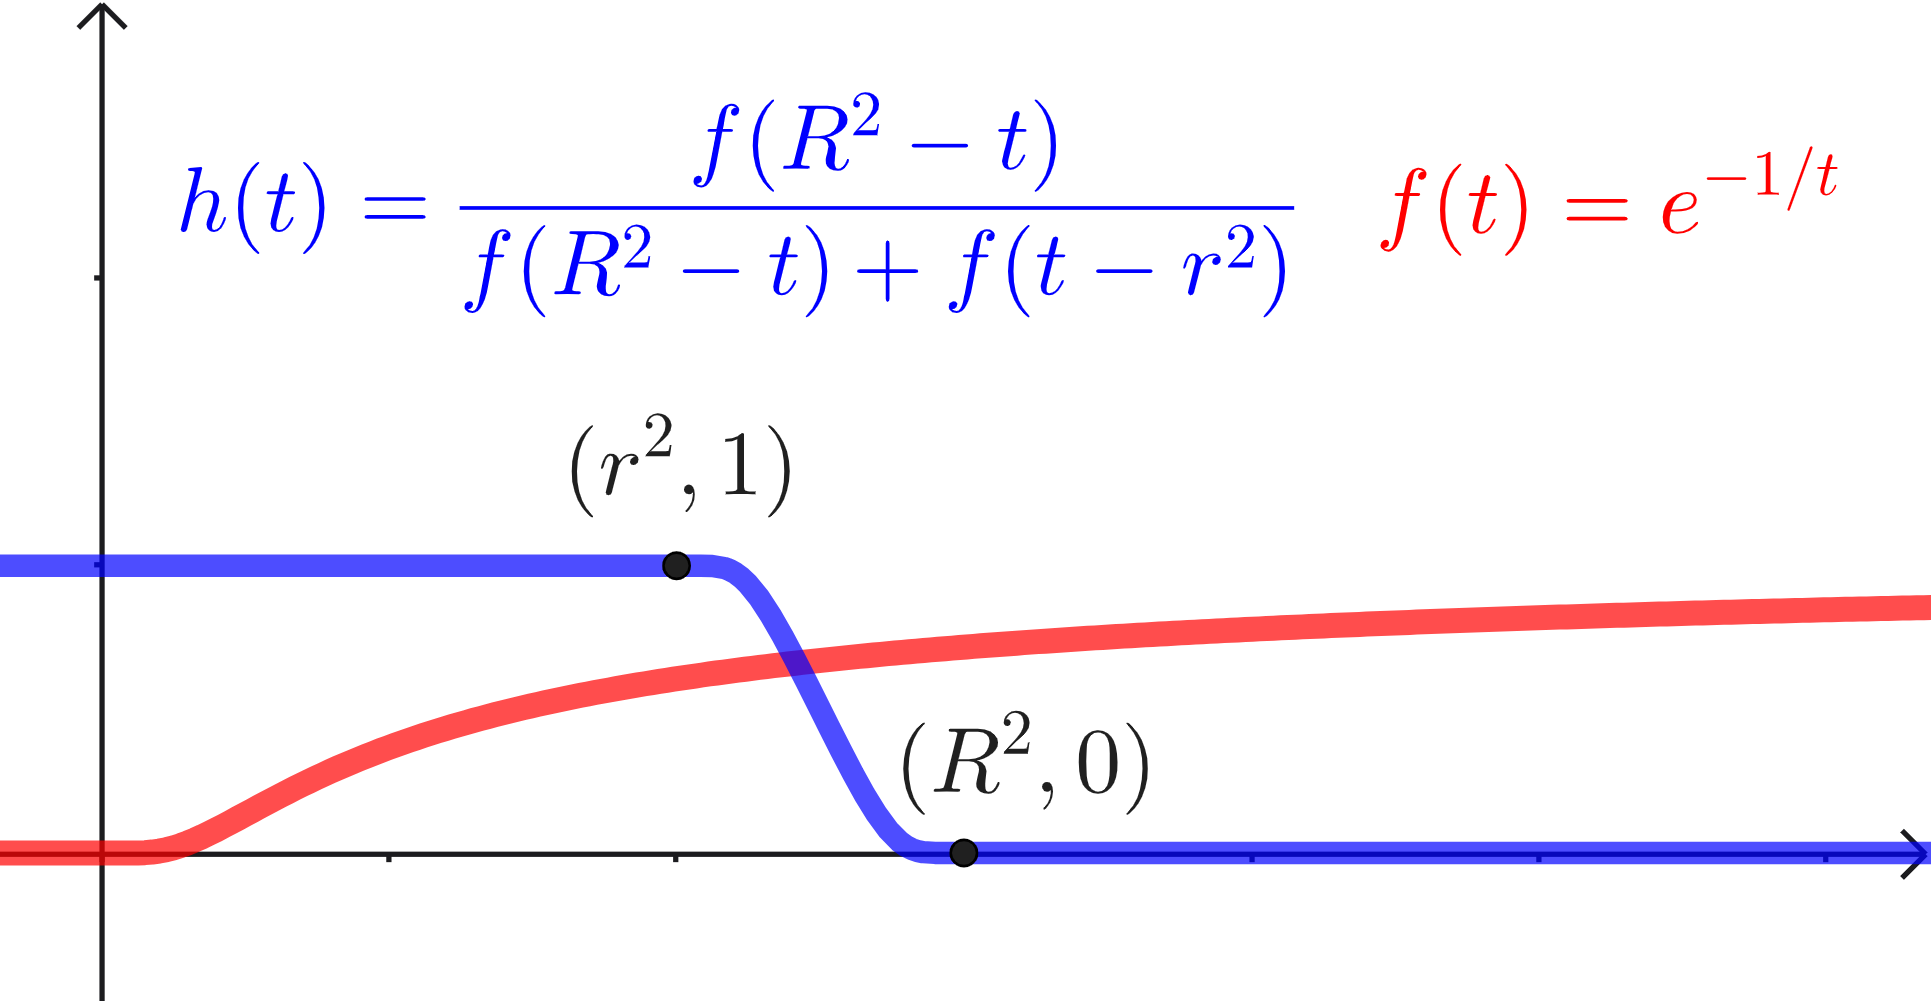
\includegraphics[width=0.5\textwidth, ]{Pictures/fh.png}
		\label{fig:fh}
		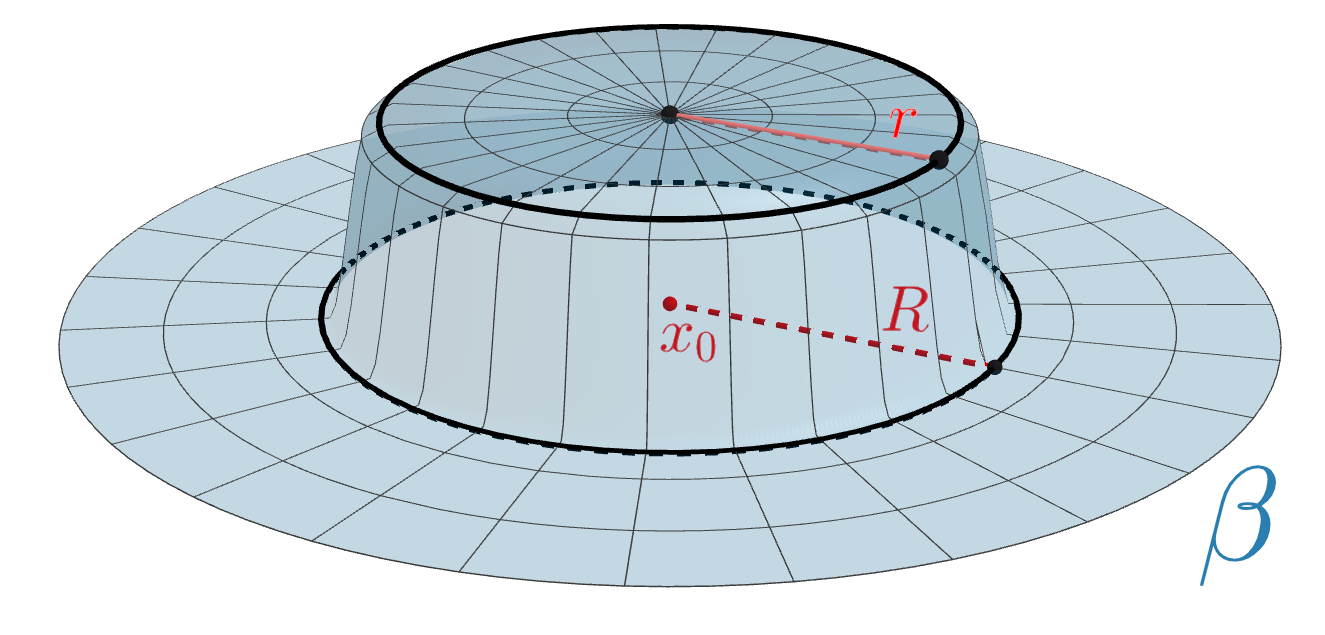
\includegraphics[width=0.5\textwidth, ]{Pictures/bump.png}
		\label{fig:bump}
\end{framed}
\end{figure}

\vspace{-15pt}

\begin{definition}
	Пусть $X$ -- метрическое пространство, $f : X \to \R$. 
	\textit{Носителем} функции $f$ называется замыкание множества точек, где функция отлична от нуля:
	\[ \operatorname{supp}(f) = \overline{\{x \in X : f(x) \neq 0\}}. \]
\end{definition}



\begin{example}
	Для функции $\beta$ имеем $\supp(\beta) = \overline{B_R(x_0)}$.
\end{example}

\begin{problem}[\textbf{лемма об исчерпывании компактами}]
	Для любого открытого множества $U$ существует семейство компактов $\{C_i\}_{i=1}^{\infty}$, такое что $C_i \subset \operatorname{int} C_{i+1}$, $\bigcup C_i = U$.
\end{problem}

\begin{lemma}
	Пусть $\{U_{\alpha}\}_{\alpha \in I}$ -- семейство открытых множеств в $\R^n$, $U = \bigcup_{\alpha \in I} U_{\alpha}$. 
	Тогда существует $\{B_i\}_{i=1}^{\infty}$ -- счетное семейство открытых шаров, такое что:
	\begin{enumerate}[itemsep = 0pt, topsep = 5pt]
		\item $\bigcup_{i=1}^{\infty} B_i = U$ (покрытие), 
		\item $\forall i \ \exists \alpha : \overline{B_i} \subset U_{\alpha}$ (вписанность), 
		\item Для каждой точки $p \in U$ есть окрестность, которая пересекается лишь с конечным числом шаров $\overline{B_i}$, то есть $\forall p \in U \ \exists U_p \subset U \ \exists N_p : \overline{B_i} \cap U_p = \emptyset \ \forall i > N_p$.
	\end{enumerate}
\end{lemma}

\begin{myproof}
	Пусть $\{C_i\}_{i=1}^{\infty}$ -- исчерпывание $U$ компактами, $C_0 = C_{-1} = \emptyset$. 
	Определим компактные <<кольца>> $K_i = C_i \setminus \operatorname{int} C_{i-1}$ для $i \geq 1$. 
	Множества $V_i = \operatorname{int} C_{i+1} \setminus C_{i-2}$ открыты и содержат $K_i$. 
	Для каждой точки $x \in K_i$ выберем открытый шар $B_x$ так, чтобы: 
	\begin{itemize}[itemsep = 0pt, topsep = 5pt]
		\item $x \in B_x$, $\overline{B_x} \subset U_{\alpha}$ для некоторого $\alpha$ и $\overline{B_x} \subset V_i$.
	\end{itemize}
	Это возможно, так как $U_{\alpha}$ открыты, $V_i$ открыто и содержит $x$. 
	Тогда семейство $\{B_x\}_{x \in K_i}$ покрывает компакт $K_i$. 
	Выделим конечное подпокрытие $\mathcal{B}_i$ и положим $\mathcal{B} := \bigcup_{i=1}^{\infty} \mathcal{B}_i$. 
	Это счетный набор шаров, покрывающий $U$. Условие вписанности выполнено по построению. 

	\vspace{5pt}
	Проверим третье свойство: <<локальную конечность>>. Пусть $p \in U$. 
	Тогда $p \in \operatorname{int} C_k$ для некоторого $k$. 
	Окрестность $U_p = \operatorname{int} C_k$ пересекается только с замыканиями шаров из семейств $\mathcal{B}_1, \dotsc, \mathcal{B}_{k+1}$. 
	Действительно, если $B \in \mathcal{B}_j$ при $j \ge k+2$, то $\overline{B} \subset V_j = \operatorname{int} C_{j+1} \setminus C_{j-2}$, а значит $\overline{B} \cap C_k = \emptyset$, так как $j-2 \ge k$.
	Поскольку каждое семейство $\mathcal{B}_i$ конечно, $U_p$ пересекается лишь с конечным числом шаров, что и требовалось.
\end{myproof}